\section{Fase 1: requisitos da avaliação}
\label{sec:fase1}

\subsection{Propósito e partes interessadas}

O propósito é \textbf{identificar, com evidências mensuráveis, os pontos fracos do SIGAA nas tarefas acadêmicas mais frequentes do estudante de graduação}, para apoiar a priorização de melhorias pela STI/UnB e embasar a ação de melhoria da Fase 4. O ponto de vista é o do estudante, com atenção a perfis vulneráveis: calouros, que desconhecem a terminologia acadêmica; estudantes que acessam o sistema apenas pelo celular; e estudantes com deficiência. Veteranos e formandos servem de contraste: problemas que persistem com experiência indicam falhas de operabilidade.

A demanda parte da disciplina FGA0315, que define o processo e os critérios de aceitação. Os resultados destinam-se à STI/UnB, operadora do sistema, que decidirá quais telas e fluxos priorizar (pelo ranking das tarefas), se investe em interface responsiva (pela Flexibilidade cruzada com o perfil de acesso) e se otimiza páginas específicas (pelo desempenho por página); ao Decanato de Ensino de Graduação e às coordenações, que decidirão quais procedimentos precisam de orientação (pelas tarefas com mais erro ou abandono); à comunidade estudantil; e à UFRN, desenvolvedora do produto.

\subsection{Produto avaliado}
\label{sec:produto}

O objeto é o \textbf{portal do discente de graduação do SIGAA/UnB}, versão v4.15.10.115 (rodapé do sistema em 16/10/2026), acessado pela interface web em produção (Fig.~\ref{fig:portal}) \cite{sigaa}. É um sistema de informação web, transacional e institucional, em JavaServer Faces, acessado pela Autenticação Integrada dos sistemas SIG. Pela classificação da IEEE 1062 apresentada na disciplina, é um produto MOTS (\textit{Modified Off-The-Shelf}): um produto-padrão da UFRN implantado com configurações próprias por instituição \cite{ramos2026processo}. Por ser de código fechado, a avaliação se restringe ao comportamento observável: é possível medir tempo de carregamento no navegador, conclusão e esforço nas tarefas, comportamento em navegadores e telas e acessibilidade, mas não o processamento no servidor, o comportamento sob carga ou a qualidade do código.

\begin{figure}[!t]
	\centering
	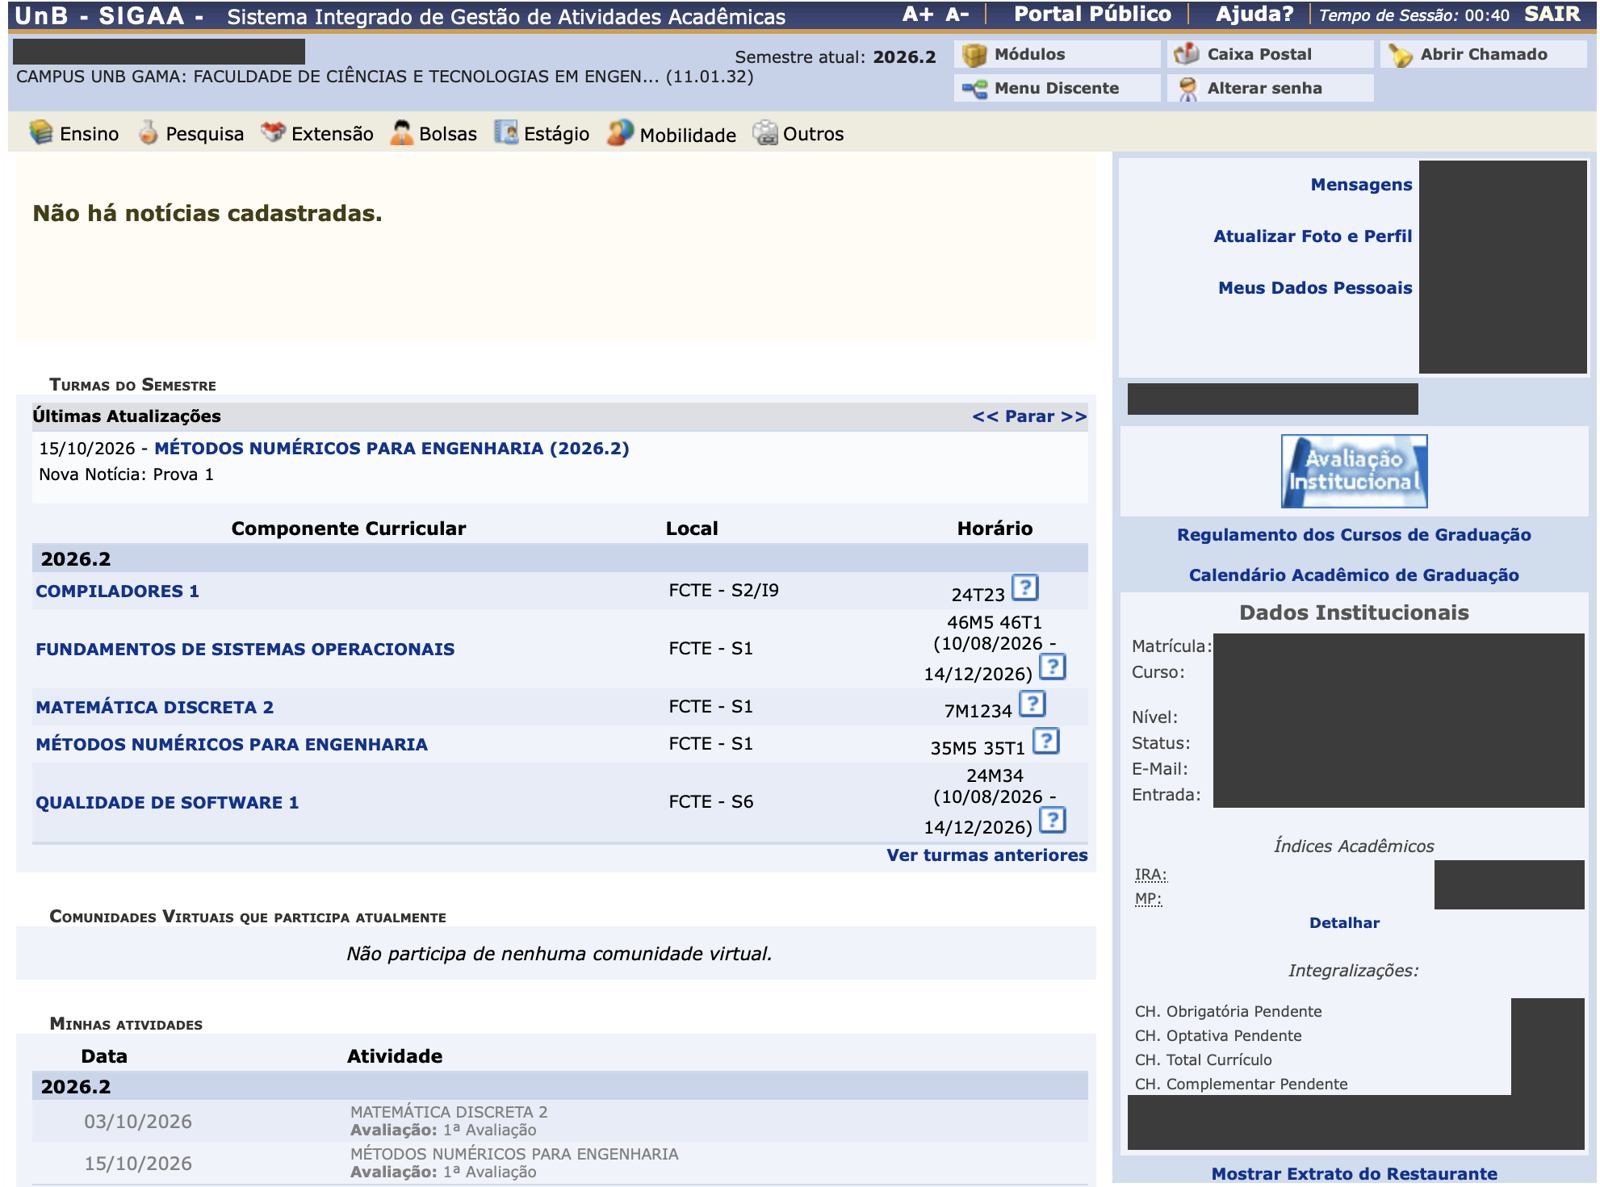
\includegraphics[width=\columnwidth]{figuras/sigaa-portal-discente.png}
	\caption{Página inicial do portal do discente do SIGAA/UnB.}
	\label{fig:portal}
	\fonte{captura da equipe em 16/10/2026, com dados pessoais ocultados.}
\end{figure}

A inspeção inicial produziu oito observações preliminares (OP), que não são resultados, mas indícios que orientaram a seleção das características (Tabela~\ref{tab:op}).

\begin{table}[!t]
	\caption{Observações preliminares da interface}
	\label{tab:op}
	\centering
	\footnotesize
	\begin{tabularx}{\columnwidth}{L{0.75cm} Y L{2.4cm}}
		\toprule
		\textbf{ID} & \textbf{Observação} & \textbf{Característica} \\
		\midrule
		OP-01 & Horários em notação codificada (``24M34''), legível só com legenda & Cap. Interação (autodescritividade) \\
		OP-02 & Menus abertos pela passagem do ponteiro, sem equivalente para toque & Flexibilidade; Cap. Interação \\
		OP-03 & Layout de largura fixa & Flexibilidade \\
		OP-04 & Menu Ensino com cerca de 20 itens em um nível & Cap. Interação (reconhecimento) \\
		OP-05 & Duas estruturas de navegação (portal e Turma Virtual) & Cap. Interação (operabilidade) \\
		OP-06 & Sessão que expira por inatividade & Cap. Interação (proteção contra erros) \\
		OP-07 & Ferramentas comunitárias para planejar o fluxo de disciplinas & Adequação Funcional (completude) \\
		OP-08 & Ampliação de fonte (A+/A-) no cabeçalho (ponto positivo) & Cap. Interação (inclusividade) \\
		\bottomrule
	\end{tabularx}
	\fonte{elaborado pela equipe.}
\end{table}

\subsection{Modelo de qualidade e priorização}
\label{sec:priorizacao}

O modelo da ISO/IEC 25010:2023 foi adaptado por três filtros: relevância para as partes interessadas, mensurabilidade em avaliação caixa-preta e viabilidade ética (nenhum teste pode alterar dados reais ou sobrecarregar a produção). Para escolher de três a quatro características, cada membro atribuiu notas de 1 a 5 de \textbf{impacto} ($I$), a consequência de uma deficiência, e de \textbf{risco} ($R$), a probabilidade de deficiência estimada pelas OP, pela idade da tecnologia e por relatos dos estudantes. A prioridade é $P = I \times R$, e foram selecionadas as características viáveis com $P \geq 15$ (Tabela~\ref{tab:matriz}).

\begin{table}[!t]
	\caption{Matriz Impacto $\times$ Risco}
	\label{tab:matriz}
	\centering
	\footnotesize
	\begin{tabularx}{\columnwidth}{L{2.25cm} C{0.2cm} C{0.2cm} C{0.35cm} Y}
		\toprule
		\textbf{Característica} & $I$ & $R$ & $P$ & \textbf{Decisão} \\
		\midrule
		Cap. de Interação & 5 & 5 & \textbf{25} & Selecionada (1): seis das oito OP \\
		Adequação Funcional & 5 & 4 & \textbf{20} & Selecionada (2): dados afetam decisões (OP-07) \\
		Efic. de Desempenho & 4 & 4 & \textbf{16} & Selecionada (3): pesa em rede móvel \\
		Flexibilidade & 4 & 4 & \textbf{16} & Selecionada (4): OP-02 e OP-03 \\
		Confiabilidade & 4 & 3 & 12 & Preterida: falhas na matrícula, fora da coleta \\
		Segurança & 5 & 2 & 10 & Inviável: exigiria testes de invasão \\
		Manutenibilidade & 3 & 3 & 9 & Inviável: sem código-fonte \\
		Compatibilidade & 2 & 2 & 4 & Preterida: não observável \\
		Seg. Operacional & 1 & 1 & 1 & Não se aplica \\
		\bottomrule
	\end{tabularx}
	\fonte{elaborado pela equipe.}
\end{table}

Nas características selecionadas, foram removidas as subcaracterísticas não mensuráveis no contexto: engajamento e assistência ao usuário (Capacidade de Interação), capacidade (Eficiência de Desempenho, por exigir testes de carga) e instalabilidade, substituibilidade e escalabilidade (Flexibilidade). O custo dessa seleção é que a avaliação descreve a qualidade do sistema em uso pelo estudante, e não a robustez interna da implementação.

\subsection{Escopo, tarefas e rigor}
\label{sec:escopo}

A avaliação usa seis tarefas representativas, escolhidas por frequência, criticidade e disponibilidade na coleta (Tabela~\ref{tab:tarefas}), executadas nos navegadores Chrome, Firefox, Safari e Edge, em telas de cerca de 360, 768 e 1280~px, e em rede comum e móvel simulada.

\begin{table}[!t]
	\caption{Tarefas representativas}
	\label{tab:tarefas}
	\centering
	\footnotesize
	\begin{tabularx}{\columnwidth}{C{0.35cm} Y L{2.7cm}}
		\toprule
		\textbf{ID} & \textbf{Tarefa} & \textbf{Caminho no sistema} \\
		\midrule
		T1 & Consultar as notas de uma disciplina & Ensino $>$ Consultar Notas \\
		T2 & Identificar dia, horário e local de uma turma & Página inicial $>$ Turmas \\
		T3 & Emitir atestado de matrícula ou histórico & Ensino $>$ Emitir Atestado \\
		T4 & Verificar índices e carga horária pendente & Ensino $>$ Índices Acadêmicos \\
		T5 & Acessar material na Turma Virtual & Turma Virtual $>$ Materiais \\
		T6 & Consultar o calendário acadêmico & Ensino $>$ Calendário \\
		\bottomrule
	\end{tabularx}
	\fonte{elaborado pela equipe.}
\end{table}

Ficam fora do escopo os portais de docentes e servidores, a pós-graduação, matrícula e trancamento (que alterariam dados reais), os demais sistemas SIG e os testes de carga e de segurança. O rigor é \textbf{intermediário}: a avaliação apoia decisões de priorização, sem impacto sobre segurança ou finanças, e é garantido por métricas objetivas, critérios fixados antes da coleta, medições repetidas e dois avaliadores nas inspeções. A amostra de conveniência, concentrada na FCTE, a versão do sistema e o período de coleta são declarados como limites de validade. A avaliação também se relaciona às metas 4.3, 10.2 e 16.6 dos Objetivos de Desenvolvimento Sustentável \cite{onu2015,ipea2018}: a permanência no ensino superior depende do sistema, estudantes de menor renda dependem mais do celular e de redes móveis, e o indicador 16.6.2 mede a satisfação com serviços públicos.
